% status: 100
% chapter: Security

\title{Apache Milagro}


\author{Arnav Arnav}
\affiliation{%
  \institution{Indiana University
  Bloomington} \city{Bloomington} \state{Indiana} \postcode{47408} \country{USA}
  }
\email{aarnav@iu.edu}

% The default list of authors is too long for headers}
\renewcommand{\shortauthors}{Arnav}


\begin{abstract}
An increasing number of devices and applications rely on cloud-based
app-centric services. Most of these application, such as Internet of
Things (IoT) applications rely on traditional Public Key
Infrastructure (PKI), to securely communicate the data. It is known
that PKI infrastructure has problems and is not the best solution as
the number of connected devices increases.  Apache Milagro provides a
distributed and scalable multi factor authentication that is ideal for
app-centric services.
\end{abstract}

\keywords{hid-sp18-503, Milagro, cryptography, cloud applications, IoT }
%use up to 5 keywords

\maketitle


\section{Introduction}

With the increasing competition in the industry, fast delivery of
services to users is one of the major concerns. Starting up services
with traditional cloud Infrastructure as a Service (IaaS) platforms
can be challenging since a bulk of the work needed to set up and
deploy an application is left for the user. With the increase in
application centric cloud computing, the developers do not need to
worry about all of the networking
issues~\cite{hid-sp18-503-bmc-app-centric}. An application centric
cloud computing environment abstracts away the complexities of
different cloud environments, allowing the developers need to manage
specific tasks related to the application and not the individual
servers themselves, thus enabling developers to spend more time to
improve the overall user experience. Most IoT applications benefit
from application centric clouds as the connected devices are part of a
common application~\cite{hid-sp18-503-vb-app-centric}.

In view of this, it is important to ensure security in the cloud. With
most of the services using password based authentication, which is
inherently vulnerable, it is important to use other information to
authenticate users properly. Multi Factor Authentication (MFA) allows
users to establish their identity by providing evidence for two out of
three requirements- knowledge (something the user knows), possession
(something the user has) and inherence (something the user
is)~\cite{hid-sp18-503-centrify-mfa}.

Apache Milagro~\cite{hid-sp18-503-milagro-website} is an Apache
incubator project that provides an open source, distributed,
certificate less security solution for cloud based application that is
easy to scale. Milagro consists of Apache Milagro Crypto Library
(AMCL) that allows users to establish distributed trust systems using
proven and tested protocols. Applications can then build on AMCL and
provide multifactor authentication using Milagro MFA, secure
communications between a client and a server and also in peer to peer
comunication~\cite{hid-sp18-503-milagro-docs-overview}.



\section{Problems with PKI}
Public Key Infrastructure has had many problems and has faced various
threats over the years.  Firstly, PKI has too many moving parts, and
setting up a PKI service is not a trivial task. This has lead to many
organizations not deploying PKI correctly and leaving their systems
vulnerable. Furthermore, most applications and users ignore PKI
warnings such as a website not being secure. These warnings and errors
can not be enforced in web browsers now, otherwise, a lot of pages and
services would stop working~\cite{hid-sp18-503-cso-pki-problems}.

Since distributing the list of revoked certificates to the whole
system can take a long time, there is no guarantee that a key belongs
to a well identified user at any time. Users may have certificates
from different Certificate Authorities, which makes it difficult to
identify users that have revoked certificates form some Certificate
Authorities~\cite{hid-sp18-503-distlab-pki-problems}.  There have been
attacks on PKI Certificate Authorities (CAs) and various CAs have been
compromised. Not only this, attackers in the past have been successful
in stealing website certificates, and code signing certificates as in
the case of
stuxnet~\cite{hid-sp18-503-securityweek-ssl-threats}. Encryption makes
initiating an SSL connection a heavyweight process and thus SSL
protected services are susceptible to attacks such as Denial of
Service (DoS) and Distributed Denial of Service (DDoS). Many such
attacks on PKI have been listed
in~\cite{hid-sp18-503-cacert-wiki-pki-history}.  Many commercial PKI
services use Identity certificates to side-step the concern whether a
commercial CA actually had the authority to provide certificates, and
leave it to the users to verify the actual
identity~\cite{hid-sp18-503-ten-pki-risks}.

Most password protected services rely on PKI and SSL to send passwords
over the internet. Recording passwords on a server is another problem
as password servers can be attacked and passwords can be stolen even
if PKI and SSL are working properly. A more philosophical issue with
centralized PKI is that user identification information lies with
centralized servers and not users
themselves~\cite{hid-sp18-503-distlab-pki-problems}. Various
approaches have been proposed to avoid some of these errors, none of
which have been widely accepted. Google has proposed an enhancement to
PKI as they suspect that PKI may be broken in the future and attackers
can use this to decipher recorded messages from old
communications~\cite{hid-sp18-503-securityweek-ssl-threats}.  Many of
these problems can be avoided by adopting a decentralized approach.


\section{Milagro Details}
% more on elliptic curve pairing -- medium
Milagro uses cryptography techniques based on pairing on elliptic
curves. Elliptic curves are mathematical structures on which
operations are easily defined. Multiplication of a point on a curve to
a number can be easily computed, but it is computationally difficult
to find the multiplier even if the result is known. This makes it
difficult to break the system while using smaller multipliers as
compared to RSA based encryption which requires the generation of
large prime numbers~\cite{hid-sp18-503-milagro-concepts}. This removes
the need to maintain and distribute certificates, thus eliminating the
need for a centralized certificate authority.

Apache milagro uses pairing based cryptography (PBC) to split a users
key among different distributed trust authorities (D-TAs) and provides
additional security as the D-TAs are isolated and independent of each
other as shown in figure~\ref{f:fig1}. This eliminates a single point
of failure and allows the key generation and distribution to be a part
of the system itself. Apache milagro provides Identity Based
Encryption (IBE) where a key can be set to a predefined identifier,
and zero knowledge authentication, where the identity of a user can be
proved without showing the user's key.  These cryptographic operations
are handled by the AMCL~\cite{hid-sp18-503-milagro-concepts}.

\begin{figure}[!ht]
  \centering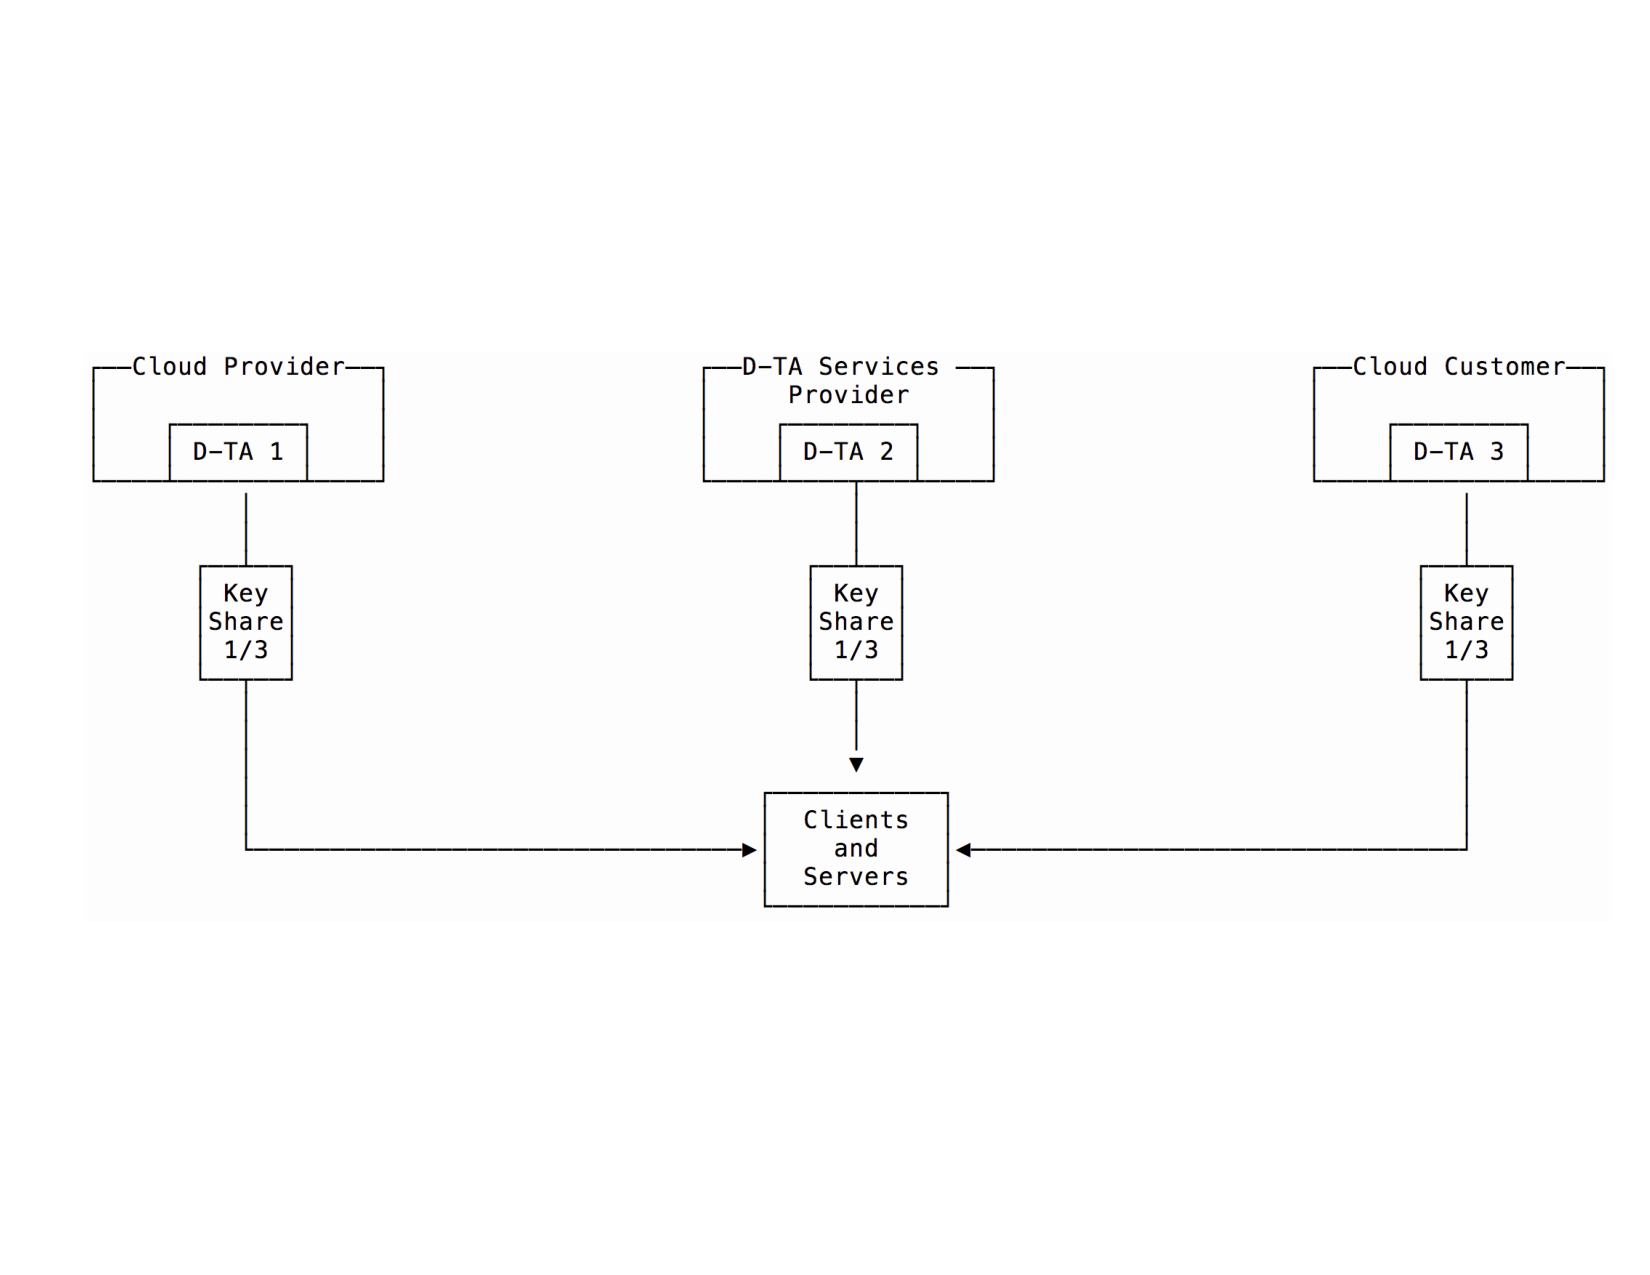
\includegraphics[width=\columnwidth]{images/dta.pdf} \caption{Each
  of the D-TAs have a fraction of the
  key~\cite{hid-sp18-503-dta-image} }\label{f:fig1}
\end{figure}

\section{Apache Milagro Crypto Library}
Despite extensive research in cryptography, most of the industry
relies on old technology for security solutions. There are many
libraries available that provide new cryptographic methods that
attempt to solve the issues in PKI\@. Most of these libraries are not
easy to use or are dependent on other
libraries~\cite{hid-sp18-503-mcl-white-paper}.

Apache Milagro crypto library is self contained and only depends on
external processes to add randomness to the key generation
process. The library is portable as it is not written in assembly
language and is reasonably fast. The library has been created keeping
in mind the memory restrictions on small connected devices and takes
minimum space. AMCL is available in many languages namely C, Java,
Javascript, Swift and Go, and uses general programming constructs
avoiding language specific functions. This allows the library to be
translated to most other languages using already available
translators~\cite{hid-sp18-503-mcl-white-paper}.

AMCL uses 128-bit AES encryption since it is the current standard for
cryptography and works as well as other variants like 256-bit AES, or
192-bit AES\@. Apart from this, the library uses ``SHA256 for hashing,
256-bit prime field elliptic curves for public key protocols, and
256-bit BN curves to support pairing-based protocols. However three
different parameterizations of elliptic curve are supported -
Weierstrass, Edwards and Montgomery, as each is appropriate within its
own niche''~\cite{hid-sp18-503-mcl-white-paper}. The library borrows
random number generation and symmetric encryption functions from the
open source MIRACL library~\cite{hid-sp18-503-mcl-white-paper}.


\section{Milagro MFA}

Milagro Multi Factor Authentication is an Apache licensed version of
the M-Pin protocol and is safe against man in the middle and key
compromise impersonation attacks~\cite{hid-sp18-503-milagro-mfa}.

Under the M-Pin protocol, the client and the server are issued secret
keys derived from their identities. The client then uses a zero
knowledge proof protocol to prove to the server that it has the secret
key. The keys are not generated at a centralized server but by various
independent D-TAs. Each part of the key (factor) is generated using
pairing on elliptic curves and is a point on the curve. The key can be
regenerated by adding the two parts together. One part of the key can
be a 4 digit pin that the user knows and the other can be an
authentication token saved on a device that a user has. Thus enabling
distributed two factor authentication. The keys are generated only at
the server and the client. The M-Pin protocol ensures forward secrecy,
so that, if long term keys are compromised, the previous session can
not be decrypted~\cite{hid-sp18-503-milagro-protocols}.


To set up a Milagro MFA service, first the crypto libraries need to be
cloned and built. Then, the credentials can be obtained by a python
script provided in the repository.  Once this is done, the distributed
trust authorities need to be set up along with a relaying party
service and a relaying party application that allows users to log
in. The Milagro repository provides scripts for these tasks. Then,
various clients can connect and user the service, with the help of
SDKs available. The SDKs are available for Android, Microsoft and iOS
platforms, and Milagro MFA can be integrated easily in web
applications easily~\cite{hid-sp18-503-mfa-install}.


\section{Milagro TLS}

Milagro TLS uses pairing based cryptography to achieve mutually
authenticated key agreement. It uses two different modules,
Milagro\_CS which uses the M-Pin protocol to establish mutual
authentication between a server and a client, and Milagro\_P2P which
uses the Chow-Choo protocol for key exchange in peer to peer
communication~\cite{hid-sp18-503-mtls-white-paper}.


The Chow-Choo protocol is an identity based key management protocol
that uses important concepts form elliptic cure pairing based
cryptography. The protocol helps Milagro to achieve MFA, key agreement
and distribution of keys from the
D-TAs~\cite{hid-sp18-503-milagro-protocols}.


As mentioned before, Milagro relies on D-TAs to issue fractions of
keys. This is possible because using a pairing on elliptic curves,
keys are generated by multiplying a master secret with a point
(P). This master secret can be easily represented as the sum of
secrets that are maintained by different D-TAs and the point (P) can
also be represented as a sum of different points representing
different factors such as a user's PIN, or a key embedded in a
device. The key in its entirety is only known by the device. If two
devices with embedded keys need to communicate with each other, they
can then calculate a common key that can be used to encrypt the
communication. Further restrictions can be enforced on the devices
where a device is allowed to send or receive data only if it is
assigned a sender or a receiver key respectively, which are two
different keys generated using fractions of keys available to each of
the devices~\cite{hid-sp18-503-milagro-protocols}.

\section{conclusion}
Traditional cryptography solutions based on Public Key Infrastructure
suffer from several problems and security threats, which have been
exploited in the past by attackers. However, PKI can still be used in
a client-server based application it is not the best solution for
distributed and peer to peer applications such as IoT applications.

Apache Milagro provides an open source, distributed and certificate
less security solution for cloud based and IoT applications. Milagro
is built on AMCL and provides Milagro MFA, which is an Apache licensed
multi factor authentication service, that can be integrated on various
platforms. Milagro also provides milagro TLS module which enables
certificate less authentication in client-server and peer-to-peer
communication.

\begin{acks}

  The authors would like to thank Dr.~Gregor~von~Laszewski for his
  support and suggestions to write this paper.

\end{acks}



\bibliographystyle{ACM-Reference-Format}
\bibliography{report} 
